\documentclass[aspectratio=169]{beamer}

\usetheme{Madrid}
\usecolortheme{default}

\usepackage{listings}
\usepackage{booktabs}
\usepackage{hyperref}
\usepackage{xcolor}
\usepackage{array}
\usepackage{graphicx}

% Code listing style
\lstset{
    basicstyle=\ttfamily\small,
    breaklines=true,
    backgroundcolor=\color{gray!10},
    keywordstyle=\color{blue},
    commentstyle=\color{green!50!black},
    stringstyle=\color{red!70!black},
    showstringspaces=false
}

\title{AI for Teaching, Learning and Collaborating}
\subtitle{D-Lab AI Pulse Workshop}
\author{}
\date{}

\begin{document}

\begin{frame}[plain]
    \titlepage
\end{frame}

% =============================================================================
% INTRODUCTION: BOTTLENECKS
% =============================================================================

\begin{frame}{The Bottleneck: Learning}
    \textbf{The traditional model:} One instructor, dozens of students, teaching ``by the average.''

    \vspace{1em}
    \textbf{What this looks like in practice:}
    \begin{itemize}
        \item A student is stuck on a concept --- office hours are five days away
        \item Course evaluations where half say ``too fast,'' the other half say ``too slow''
        \item A grad student spends weeks reading dozens of papers for a new project, only to discover the idea isn't novel
    \end{itemize}

    \vspace{1em}
    Material is presented at one pace, in one way. Students who need more time wait. Students who need less time disengage.
\end{frame}

\begin{frame}{The Bottleneck: Teaching \& Collaborating}
    \textbf{Teaching:}
    \begin{itemize}
        \item Instructors spend more time on \LaTeX{} and preparing problem sets than on improving the syllabus
        \item GSIs answer the same email 30 times: ``Where is the rubric?'' ``Can I submit late?'' ``How do I request DSP accommodations?''
    \end{itemize}

    \vspace{1em}
    \textbf{Collaborating:}
    \begin{itemize}
        \item People leave a research group meeting and disagree on who's doing what and when it's due
        \item Co-authors have partial results, drafts, and notes scattered across email threads, Google Docs, and Slack --- no single source of truth
    \end{itemize}
\end{frame}

\begin{frame}{A New Paradigm?}
    \textbf{Personalized education:}
    \begin{itemize}
        \item Students use AI as a tutor --- navigate material at their own pace, get unstuck immediately
        \item Instructors are freed from repetitive tasks --- focus on updating content, advising students, higher-level work
        \item Teams get shared AI workspaces that capture decisions, assign tasks, and maintain a single source of truth
    \end{itemize}

    \vspace{1em}
    \textbf{Today:} Tools that are making this possible right now.

    \vspace{1em}
    \textbf{Tools:} NotebookLM, Notion AI, Otter AI

    \vspace{0.3em}
    \textbf{In passing:} Curipod, Mizou, Mural
\end{frame}

\begin{frame}{Today's Roadmap}
    \textbf{1. NotebookLM}
    \begin{itemize}
        \item Source-grounded AI: your documents, not the internet
        \item Rapid-fire feature tour + the ``Bureaucratic Agent''
    \end{itemize}

    \vspace{0.8em}
    \textbf{2. Learning \& Research}
    \begin{itemize}
        \item Using NotebookLM for literature reviews and research
        \item Teaching tools: Curipod \& Mizou
    \end{itemize}

    \vspace{0.8em}
    \textbf{3. Collaborating}
    \begin{itemize}
        \item Notion AI: writing, meeting notes, agents, calendar
        \item Otter AI: transcription and cross-meeting intelligence
    \end{itemize}

    \vspace{0.8em}
    \textbf{Live demos throughout.}
\end{frame}

% =============================================================================
% NOTEBOOKLM DEEP DIVE
% =============================================================================

\begin{frame}{What is NotebookLM?}
    \textbf{Google's source-grounded AI} powered by Gemini

    \vspace{1em}
    \textbf{Key differentiator:} Answers come from \textit{YOUR documents}, not the internet.

    \vspace{1em}
    \textbf{How it works:}
    \begin{itemize}
        \item Upload papers, lecture notes, syllabi, or any documents
        \item AI generates content \textit{grounded} in those sources
        \item Every claim is traceable back to your materials
        \item No hallucinated information from external training data
    \end{itemize}

    \vspace{1em}
    \textbf{Also:} Can search the web for new sources and add them to your notebook

    \vspace{0.5em}
    \textbf{Free to use:} \url{https://notebooklm.google.com/}
\end{frame}

\begin{frame}{NotebookLM: What Can It Do?}
    \textbf{From your uploaded sources, NotebookLM can generate:}

    \vspace{0.8em}
    \begin{columns}[T]
    \begin{column}{0.48\textwidth}
        \begin{itemize}
            \item Chat with an AI agent
            \item Summaries \& reports
            \item Audio overviews (``podcasts'')
            \item Mind maps
            \item Flashcards
        \end{itemize}
    \end{column}
    \begin{column}{0.48\textwidth}
        \begin{itemize}
            \item Quizzes
            \item Slide decks
            \item Study guides
            \item Search for new sources
        \end{itemize}
    \end{column}
    \end{columns}

    \vspace{1em}
    \textbf{Sharing:} Notebooks can be shared --- students making study groups, professors sharing resources

    \vspace{0.8em}
    \textbf{Demo:} 30-second tour of each feature
\end{frame}

\begin{frame}{The ``Bureaucratic Agent''}
    \textbf{Upload institutional documents $\rightarrow$ instant Q\&A for common questions}

    \vspace{1em}
    \textbf{Example:} Upload the syllabus + UC Berkeley regulations on:
    \begin{itemize}
        \item Academic integrity and cheating policies
        \item How to request DSP accommodations
        \item Sickness and athletic absence policies
        \item Grading rubrics and late submission rules
    \end{itemize}

    \vspace{1em}
    \textbf{Now the GSI doesn't answer the same email 30 times.}

    \vspace{1em}
    \textbf{Other applications:}
    \begin{itemize}
        \item Lab safety rules and protocols
        \item How to use the EML SLURM server
        \item Major/minor requirements and advising
        \item How enrollment and waitlists work
    \end{itemize}
\end{frame}

% =============================================================================
% LEARNING & RESEARCH
% =============================================================================

\begin{frame}{NotebookLM for Research}
    \begin{columns}[T]
    \begin{column}{0.45\textwidth}
        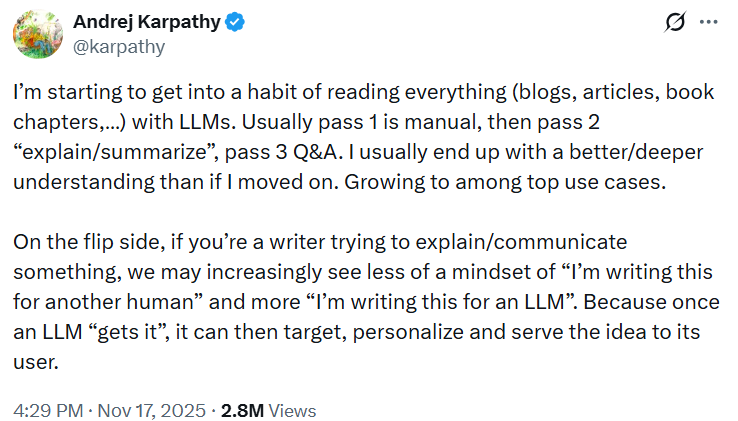
\includegraphics[width=\textwidth]{../karpathy_tweet.png}
    \end{column}
    \begin{column}{0.52\textwidth}
        \textbf{Why researchers love it:}
        \begin{itemize}
            \item Upload papers $\rightarrow$ ask questions across all of them
            \item Synthesize findings, compare methods, find contradictions
            \item Generate audio overviews for learning on the go
            \item Create mind maps of conceptual connections
        \end{itemize}

        \vspace{0.8em}
        \textbf{Especially useful for:}
        \begin{itemize}
            \item Grad students starting new projects
            \item Researchers joining new labs or switching fields
        \end{itemize}
    \end{column}
    \end{columns}
\end{frame}

\begin{frame}{Demo: Literature Review Workflow}
    \textbf{Starting a new research project with NotebookLM:}

    \vspace{1em}
    \begin{enumerate}
        \item Write a 1--2 paragraph research idea with some initial references
        \item Upload references $\rightarrow$ Ask: ``How novel is this idea?''
        \item Use search (or Perplexity) to find and add more papers
        \item Ask for synthesis of the literature as you keep writing
        \item Compare papers: ``How does Smith (2020) differ from Jones (2022)?''
        \item Generate mind maps of the conceptual landscape
    \end{enumerate}

    \vspace{1em}
    \textbf{The notebook grows with your project} --- a living literature review, not a static document.

    \vspace{0.5em}
    \textbf{[LIVE DEMO]}
\end{frame}

\begin{frame}{In Passing: Teaching Tools}
    \textbf{Curipod} --- \url{https://curipod.com/}
    \begin{itemize}
        \item AI-powered interactive lesson builder
        \item Generate polls, word clouds, open-ended prompts from your content
        \item Real-time student engagement during lectures
    \end{itemize}

    \vspace{1.5em}
    \textbf{Mizou} --- \url{https://mizou.com/}
    \begin{itemize}
        \item AI chatbot builder for educators
        \item Create custom tutoring bots grounded in your course material
        \item Students interact with the bot for practice and review
    \end{itemize}

    \vspace{1em}
    Both are free to try and designed specifically for educational settings.
\end{frame}

% =============================================================================
% COLLABORATING
% =============================================================================

\begin{frame}{Collaborating: The Problem}
    \textbf{Teams already use NotebookLM together:}
    \begin{itemize}
        \item Add partial empirical results, literature review, drafts, reports
        \item Create a unified, queryable workspace everyone can search
    \end{itemize}

    \vspace{1em}
    \textbf{But real collaboration needs more:} writing together, tracking tasks, capturing meeting decisions.

    \vspace{1em}
    \textbf{In passing --- Mural} (\url{https://mural.co/}):
    \begin{itemize}
        \item AI-assisted visual collaboration boards
        \item Brainstorming, affinity diagrams, research synthesis
        \item Useful for workshops, lab retreats, group ideation
    \end{itemize}

    \vspace{1em}
    \textbf{Next:} Notion AI and Otter AI
\end{frame}

\begin{frame}{Notion AI: Writing \& Content}
    \textbf{AI built into your workspace:}
    \begin{itemize}
        \item \textbf{Draft} --- generate first drafts from a prompt
        \item \textbf{Edit} --- improve clarity, grammar, flow
        \item \textbf{Summarize} --- condense long documents
        \item \textbf{Translate} --- switch between languages
        \item \textbf{Adjust tone} --- formal, casual, academic
        \item \textbf{Highlight text} $\rightarrow$ simplify, expand, or rewrite
    \end{itemize}

    \vspace{1em}
    \textbf{Use cases for academia:}
    \begin{itemize}
        \item Syllabi, assignments, lecture notes
        \item Workshop Q\&A documentation
        \item Connects to Slack and Google Drive
    \end{itemize}
\end{frame}

\begin{frame}{Notion AI: Agents \& Workflows}
    \textbf{Notion AI Agents} can automate recurring tasks:
    \begin{itemize}
        \item Synthesize teaching feedback and course evaluations
        \item Process survey responses for qualitative research
        \item Summarize weekly reports across a team
    \end{itemize}

    \vspace{1em}
    \textbf{Meeting Notes $\rightarrow$ Action Items:}
    \begin{itemize}
        \item AI generates meeting summaries with tasks, owners, priorities, and due dates
        \item Drag an action item from the summary into a task database
        \item Assign it to someone on your team with a due date
        \item \textbf{Key insight:} Meeting notes live \textit{inside} Notion --- action items flow directly into project databases, no export/import step
    \end{itemize}
\end{frame}

\begin{frame}[fragile]{Notion AI: Calendar Integration}
    \textbf{Notion Calendar} (as of Notion 3.1):
    \begin{itemize}
        \item Add AI Meeting Notes to calendar events
        \item View and manage Notion databases in your calendar
        \item Drag database items into your calendar grid
    \end{itemize}

    \vspace{1em}
    \textbf{The AI Agent can search your calendars:}

    \vspace{0.5em}
    \begin{lstlisting}[basicstyle=\ttfamily\small]
"When did I last meet with Steven and what
 were the action items?"
    \end{lstlisting}

    \vspace{0.5em}
    Searches across Google Calendar and Notion Calendar to answer.

    \vspace{1em}
    \textbf{The workflow:} Meet $\rightarrow$ AI captures notes $\rightarrow$ tasks assigned with due dates $\rightarrow$ project databases updated $\rightarrow$ calendar reflects new deadlines
\end{frame}

\begin{frame}{Otter AI: Where It Shines}
    \textbf{Otter vs.\ Notion for meeting transcription:}

    \vspace{0.5em}
    \begin{table}
        \centering
        \begin{tabular}{p{5.5cm}p{5.5cm}}
            \toprule
            \textbf{Otter AI} & \textbf{Notion AI} \\
            \midrule
            Speaker identification & One continuous text block \\
            Cross-meeting intelligence & Single-meeting notes \\
            Auto-joins from calendar & Manual ``Start transcribing'' \\
            Voice-activated mid-meeting & Passive transcription \\
            Captures video \& slides & Audio only \\
            Free: 300 min/month & Requires Business (\$20/user/mo) \\
            \bottomrule
        \end{tabular}
    \end{table}

    \vspace{0.5em}
    \textbf{Standout feature:} Ask Otter mid-meeting ``What did we decide about the budget last week?'' --- it pulls from past transcripts across your entire meeting history.
\end{frame}

% =============================================================================
% DISCUSSION & RESOURCES
% =============================================================================

\begin{frame}{Discussion}
    \begin{enumerate}
        \item \textbf{Is struggling the point?} If a student can ask AI to explain any concept instantly, do they lose something? Is working through difficulty how we actually learn?

        \vspace{0.5em}
        \item \textbf{CliffsNotes for everything?} Are we building deeper understanding, or are we just making it easier to skip the hard parts?

        \vspace{0.5em}
        \item \textbf{How does the instructor's role change?} If AI handles tutoring, Q\&A, and material generation --- what's left? What \textit{should} be left?

        \vspace{0.5em}
        \item \textbf{Who benefits?} Do these tools narrow or widen the gap between students who have support and those who don't?
    \end{enumerate}
\end{frame}

\begin{frame}{Resources}
    \textbf{Tools covered today:}
    \begin{itemize}
        \item NotebookLM: \url{https://notebooklm.google.com/}
        \item Notion AI: \url{https://www.notion.so/}
        \item Otter AI: \url{https://otter.ai/}
    \end{itemize}

    \vspace{0.5em}
    \textbf{Mentioned:}
    \begin{itemize}
        \item Curipod: \url{https://curipod.com/}
        \item Mizou: \url{https://mizou.com/}
        \item Mural: \url{https://mural.co/}
    \end{itemize}

    \vspace{0.5em}
    \textbf{D-Lab:}
    \begin{itemize}
        \item \url{https://dlab.berkeley.edu/}
    \end{itemize}

    \vspace{0.5em}
    \textbf{Questions?} Let's discuss!
\end{frame}

\end{document}
